\documentclass[a4paper,onecolumn,oneside,titlepage,12pt]{report}

\usepackage{listings}
\usepackage{tikz}
\usetikzlibrary{shapes,arrows}

% Define block styles for flow diagrams
\tikzstyle{decision} = [diamond, draw, fill=black!20, 
    text width=4.5em, text badly centered, node distance=3cm, inner sep=0pt]
\tikzstyle{block} = [rectangle, draw, fill=black!20, 
    text width=5em, text centered, rounded corners, minimum height=4em]
\tikzstyle{line} = [draw, -latex']
\tikzstyle{cloud} = [draw, ellipse,fill=red!20, node distance=3cm,
    minimum height=2em]

\def\tm{\leavevmode\hbox{$\rm {}^{TM}$}}

\definecolor{light_gray}{rgb}{0.8,0.8,0.8}

\title{AndroAR: Mobile Augmented Reality application}
\author{Alexandru Damian}
\date{16 June 2012}


\begin{document}
\maketitle
\begin{abstract}
ABSTRACT
\end{abstract}
\tableofcontents

\chapter{Introduction}
\section{Motivation}
\section{Structure of thesis}

\chapter{State of the Art}
Augmented Reality is very popular in the mobile applications industry. However, most applications interact very little with the video feed they overlay the information on. Typically, applications will:
\begin{itemize}
	\item interact with a small part of the current view, such as a \emph{logo} or \emph{banner};
	\item take advantage of the localization capabilities of the phone, such as \emph{GPS positioning} or \emph{compass} and place information on the screen with disregard to what the user's line of sight actually is (\emph{e.g. a user might be facing a wall and be overrun with information, even though he doesn't see anything relevant}.
\end{itemize}
\section{Layar}
Layar is a mobile application built for Android and iOS. It is the most well-known augmented reality mobile application in the industry. Having pivoted a few times, it now focuses on bringing the augmented reality experience to printed publications.
\subsection*{Disadvantages}
\begin{itemize}
	\item Layar is currently focused on printed publications. One can try to associate a current view of the world (\emph{i.e. what the user sees at a particular moment through the smartphone's camera}) with a \emph{printed magazine page}. However, the world is dynamic and tridimensional, and, therefore, problems will arise when trying to extend the Layar behavior.
\end{itemize}

We must note that Layar has limited support for 3D objects.
\section{Google Maps / Street View}
Google Maps enables users to navigate and receive directions on an extremely detailed map. Street View, a subproduct of Google Maps, allows navigation at street view level, allowing the user to asociate information with their surroundings.
\subsection*{Disadvantages}
\begin{itemize}
	\item Street View is not live. Street View imagery was captured using dedicated equipment. Efforts are being made to keep the imagery as up-to-date as possible, but this cannot be done all around the world. For example, several areas in Romania contain images that are 4 years old.
	\item Only recently has Street View been offering imagery outside of streets range (\emph{i.e. pedestrian roads, parks, campuses, indoor}
	\item Users can navigate through Street View using their smartphone, but the Street View imagery will completely replace what the user sees. This will result in \emph{lower accuracy} and \emph{higher bandwith usage}.
\end{itemize}
\section{Wikitude}

Wikitude is one of the first implementations of an augmented reality environment. Wikitude is more feature-rich than Layar, offering more than $3500$ so-called \emph{worlds} (these are basically layers of information that will be displayed on top of the current camera feed, \emph{i.e. tweets, nearby hotels, events, etc.}).

\subsection*{Disadvantages}
\begin{itemize}
	\item although there are many sources of information that can be presented to the user, 
\end{itemize}

\section{Mixare}

\chapter{Goals for AndroAR}
While designing AndroAR, we focused on several keywords:
\section*{Live}
We need to focus on displaying information relevant to what the user sees, not just to the user's position and orientation. Most augmented reality applications will place an overlay of information on top of the current camera feed; the two are related only by the current localization features of the user (\emph{i.e. GPS position, compass orientation}) and not by what the camera feed actually shows.

\textbf{Layar} offers a live view, but is only focused on paper.

\textbf{Street View} doesn't offer a live view, but Google Maps supports uploading of user images and tagging; these images can be augmented onto the Street View imagery, but that only works on the desktop web version.
\section*{Fast}
Using the camera feed brings some issues regarding speed and bandwidth since displaying information is not a matter of only querying a database with the user's current position anymore. We need to find a way to divide the computational effort between the server and the mobile application. We must also consider the effect of latency on the query replies (\emph{i.e. by the time the user receives the query reply, the detected objects might have translated).}

By its design, \textbf{Layar} users will wait for the reply to the query. A typical usecase of Layar is: \emph{a user will see the message \emph{Scan for a behind-the-scenes video of the article} on the cover of a magazine and will wait for the application to serve the video}.

Since it's not live, \textbf{Street View} can precache the information it needs in order to serve information to the user. Queries will not be affected by what the users see, but only by their position.

\section*{Correct}
We must make sure that the information (\emph{i.e. objects associated with images and metadata}) is correct. Since we are using a crowdsourced approach, we should consider rating of images to allow removal of incorrect associations. Also, we must deal with spam.

\textbf{Layar} has fewer problems with this since they are using a business-to-consumer model, in which the information is provided by the business and the queries are made by the consumer (\emph{i.e. a magazine creates the layers and the buyer uses the application}. Layar can correctly assume that business will provide high-quality information.

\textbf{Street View} already has correct and high-quality imagery. Images added by users can easily be filtered by first querying them against their database.

\chapter{System Workflow}
A user can interact with our application in two ways:
\begin{enumerate}
	\item by making queries while using the application;
	\item by sending images annotated with objects and metadata.
\end{enumerate}
We will illustrate the overall workflow for each of them below.

\section{Queries}
Let us assume that at one point in time, while the user is using the application, the applicatin needs to find all the objects that appear in a frame, along with their metadata. To accomplish this, we will send a request to the server that will be completed in the following steps:
\begin{enumerate}
	\item The mobile application will encapsulate the current frame, along with localization information (GPS position and compass orientation) and send it to the server;
	\item The server will forward the query to the database which will fetch from storage, all the possible objects in the user's line of sight.
	\item The database will return the objects that might pe present in the frame. For each object, information that will help match the particular object to an image will also be returned. Note that each object may (and should) be present in more than one image. We will return matching information for the best performing fraction of these images. The information we return may contain:
	\begin{enumerate}
		\item image features (\emph{e.g. lines, corners, areas of constrast, etc.});
		\item illumination information;
		\item etc.
	\end{enumerate}
	\item We will forward the initial query, along with the possible objects to the image recognition component. This component will:
		\begin{enumerate}
			\item compute the features for the query image;
			\item compare the features for the query image to the features of every possible object and assign a rate of success (or certainty) to each statement
			
			$X$ is present in the query image $I$, where $X$ is a $possible\:object$
		\end{enumerate}
		\item Using a threshold for the rate of success, we will end up with a subset of the possible objects being classified as detected objects. These detected objects, along with the corresponding positions in the query image will be sent back to the server by the image recognition component.
		\item The server will then forward the reply to the mobile application.
\end{enumerate}

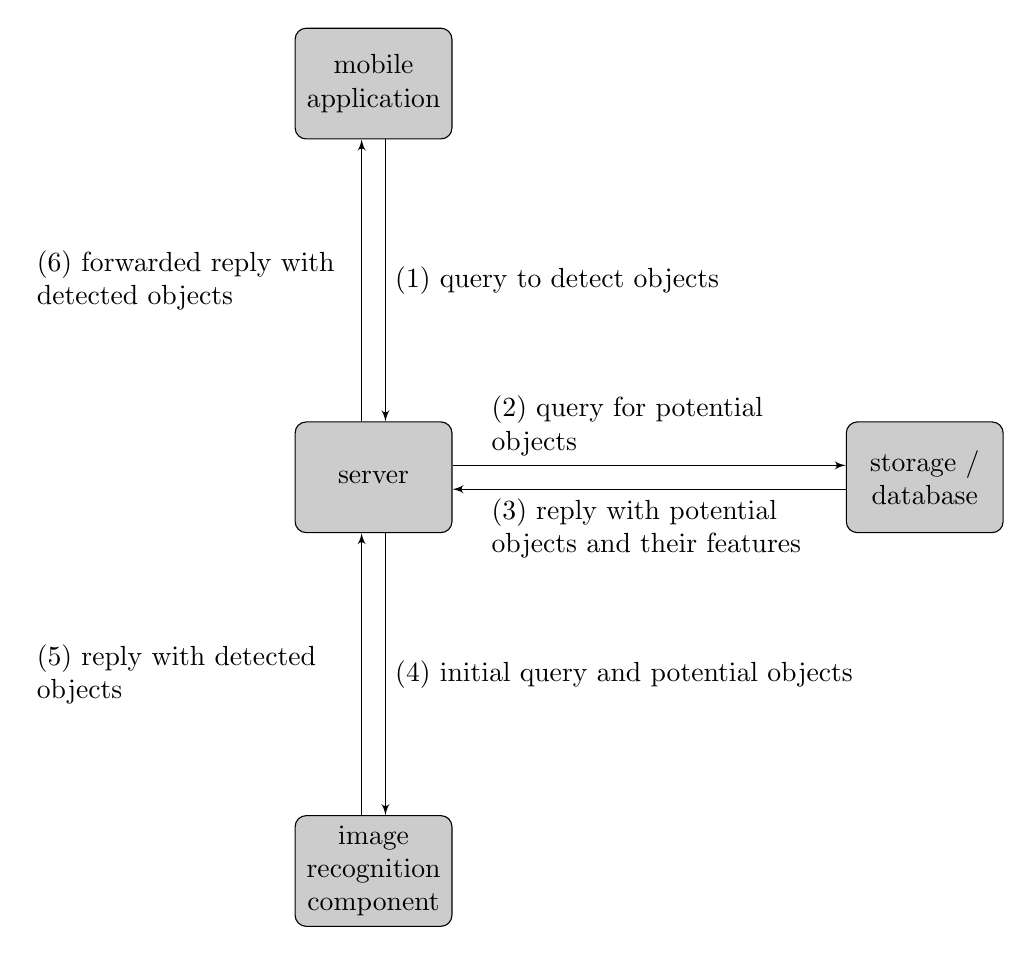
\begin{tikzpicture}[node distance = 2cm, auto]
    % Place nodes
    \node [block] (app) {mobile application};
    \node [block, below of=app, node distance=5cm] (server) {server};
    \node [block, right of=server, node distance=7cm] (db) {storage / database};
    \node [block, below of=server, node distance=5cm] (ai) {image recognition component};
    % Draw edges
    \path [line] ([xshift=1ex]app.south) -- node [text width=6cm] {(1) query to detect objects} ([xshift=1ex]server.north);
    \path [line] ([yshift=1ex]server.east) -- node [text width=4cm] {(2) query for potential objects} ([yshift=1ex]db.west);
    \path [line] ([yshift=-1ex]db.west) -- node [text width=4cm] {(3) reply with potential objects and their features} ([yshift=-1ex]server.east);
    \path [line] ([xshift=1ex]server.south) -- node [text width=6cm] {(4) initial query and potential objects} ([xshift=1ex]ai.north);
    \path [line] ([xshift=-1ex]ai.north) -- node [text width=4cm] {(5) reply with detected objects} ([xshift=-1ex]server.south);
    \path [line] ([xshift=-1ex]server.north) -- node [text width=4cm] {(6) forwarded reply with detected objects} ([xshift=-1ex]app.south);
    
\end{tikzpicture}

\subsection*{Example}
We will illustrate the previous workflow with an example:
\begin{itemize}
	\item Let us assume that a tourist is travelling through Paris and, when a query is made to the server, he is looking at the \emph{Eiffel Tower}.
	\item The server will receive a query containing an image of the \emph{Eiffel Tower}, along with the tourist's position and orientation. 
	\item The server will then request from the database, the possible objects that might be present in the tourist's line of sight. For example, the server might request the top (at most) 10 ranking instances of all the objects in a 1 kilometer radius and in a 90\% cone in front of the user.
	\item A possible reply from the server contains the features for 10 images of the \emph{Eiffel Tower} and the features for 6 images of \emph{Les Invalides}.
	\item These will be forwarded to the image recognition component which will try to match 2 possible objects with the query image. The confidence rates that result can be:
		\begin{center}
			\begin{tabular}{|c|c|}
				\hline
				\textbf{Object} & \textbf{Confidence}\\
				\hline
				Eiffel Tower & .85\\
				Les Invalides & .5\\
				\hline
			\end{tabular}
		\end{center}
	\item With a threshold of $.75$, only the \emph{Eiffel Tower} will be selected as a valid match and that will be returned as the query reply.
\end{itemize}

\section{Store requests}
Our application supports and encourages crowd-sourced contributions to annotate new landmarks. Should a user want to annotate a landmark, the application will allow them to freeze on a particular frame, create  bounding boxes around the landmarks and annotate them with information. We will need to store this information into our database.

To accomplish this, we will send a request to the server that will be completed in the following steps:
\begin{enumerate}
	\item The mobile application will encapsulate the current frame, along with localization information (GPS position and compass orientation) and the bounding boxes and metadata for each input object; it will then send this request to the server.
	\item The server will forward the request to the database which will store the data (\emph{i.e. image, localization, objects ids, objects metadata, objects cropped images, etc.}).
	\item The server will then forward the request to the image recognition component which will compute the features for:
	\begin{itemize}
		\item the large image;
		\item the small images (\emph{i.e. the cropped images using the provided bounding boxes for the detected objects}).
	\end{itemize}
	\item The image recognition component will then send them back to the server.
	\item The server will forward them to the database, which will store them.
\end{enumerate}

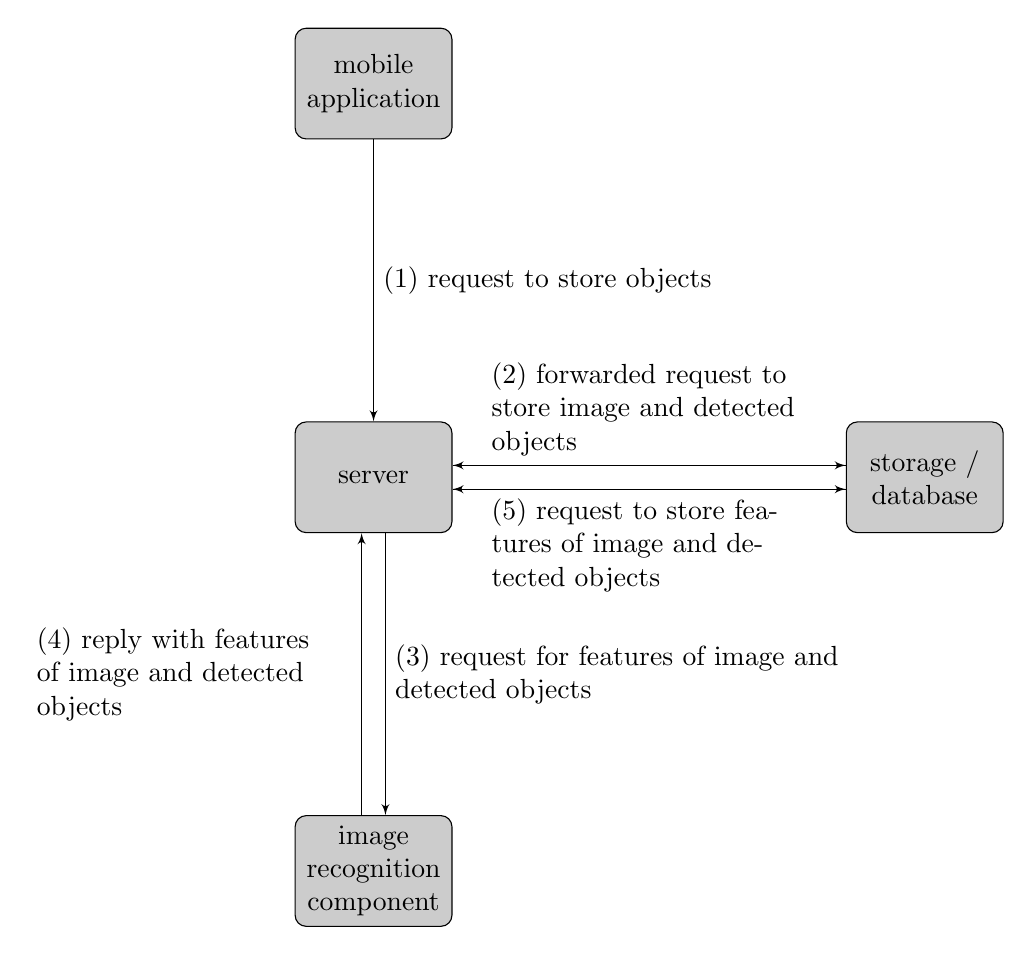
\begin{tikzpicture}[node distance = 2cm, auto]
    % Place nodes
    \node [block] (app) {mobile application};
    \node [block, below of=app, node distance=5cm] (server) {server};
    \node [block, right of=server, node distance=7cm] (db) {storage / database};
    \node [block, below of=server, node distance=5cm] (ai) {image recognition component};
    % Draw edges
    \path [line] (app) -- node [text width=6cm] {(1) request to store objects} (server);
    \path [line] ([yshift=1ex]server.east) -- node [text width=4cm] {(2) forwarded request to store image and detected objects} ([yshift=1ex]db.west);
    \path [line] ([yshift=1ex]db.west) -- ([yshift=1ex]server.east);
    \path [line] ([xshift=1ex]server.south) -- node [text width=6cm] {(3) request for features of image and detected objects} ([xshift=1ex]ai.north);
    \path [line] ([xshift=-1ex]ai.north) -- node [text width=4cm] {(4) reply with features of image and detected objects} ([xshift=-1ex]server.south);
    \path [line] ([yshift=-1ex]server.east) -- node [below, text width=4cm] {(5) request to store features of image and detected objects} ([yshift=-1ex]db.west);   
    \path [line] ([yshift=-1ex]db.west) -- ([yshift=-1ex]server.east);
    
\end{tikzpicture}

\chapter{Performance issues}
The workflows presented in the previous section pose several performance issues.
\section{Query issues}
Ideally, we would want to answer queries at a rate equal to the \emph{fps} value of the current video feed. A sufficient value for the \emph{fps} would be $5-10$. We do not need the performance of a higher \emph{fps} value (\emph{i.e. the cinematic value of 24}).

However, even intuitively, it will be extremely difficult to answer queries at a rate of $5-10$ \emph{fps}, for \emph{each} connected client. Moreover, we must consider the limited amount of traffic a mobile phone has available on 3G / 4G networks. Keeping this in mind, we should limit the amount of queries issued by the client.

\subsection{Sparse Queries}
We can achieve a good trade-off between quality and performance by using a simple observation: \emph{in most scenarios, a detected building will not disappear from the user's line of sight in less than $1-2$ seconds}; that is because the user will not pan the camera fast enough so that the entire landscape changes.

We can implement this by:
\begin{enumerate}
	\item issuing sparse queries (\emph{i.e. a query every 5 seconds});
	\item in between these queries, using the orientation (mainly) and the GPS position of the device to translate or scale the bounding boxes accordingly;
\end{enumerate}
We should note that:
\begin{enumerate}
	\item there will be a delay between the moment the query is issued and the moment the response is received; we should translate and scale the bounding boxes according to the relative move of the device;
	\item translation and scaling according to localization capabilities will allow for higher quality user experience; let us imagine that the user is looking at a building for which the right half is very rich in features and the left side is very poor in features, and that the building is correctly detected. Should the user pan the camera to the left and have only the left half of the building visible, in the $5$ second range, a bounding box will still be shown around the building.
\end{enumerate}
We will also ilustrate this in a future chapter, but it important to note why we chose the $5$ second range. Using a simple implementation with the following features:
\begin{itemize}
	\item \emph{SURF} detector;
	\item \emph{Brute-force} matcher;
	\item 2 potential objects (totalling 4 instances)
\end{itemize}
the average round-trip time for a query was $3.5$ seconds, using a \emph{high-quality, color, 8 megapixel} image.

\subsection{Caching}
Given that the users will change their GPS position so sightly every-time a query is issued (\emph{i.e. a typical user will travel by foot; assuming their average speed is $4 km/h$, they will travel $1 meter$ every second, which is roughly $.03 degree seconds$}), we can take full advantage of \emph{caching}. We could query the database for \emph{all} the objects surrounding  the users, not just those in their cone of sight and cache their features. Should the user move, we only need to query the database for the objects in the areas previously not covered.

\section{Storage issues}

We stated above, we are using a crowdsourced approach to getting new data. However, this is often not enough, since most of the users will submit very little information.

\subsubsection{Retrieving more examples}

We have come up with some ideas to increase the number of correct examples (\emph{i.e. object instances}) that are saved to our database:
\begin{enumerate}
	\item when a user freezes a frame and tags several objects, we can safely assume that some frames before and some frames after will contain that object. We can therefore send a batch of frames to the server to store in the database. The server should decide which of them it should keep (\emph{i.e. frames that actually contain the object and have good quality, and are not repetitive};
	\item when a mobile application instance issues a query and that query returns a reply that contains objects rated with high confidence, than we can also assume that some frames before and some frames after will contain those objects. We can then proceed as above.
\end{enumerate}


\chapter{Implementation}
\section{Server}
The server must be able to deal with the following aspects:
\begin{enumerate}
	\item be easy to distribute;
	\item allow multiple, simultaneous remote connections;
	\item easily implement an interface with the database;
	\item implement or interface with the image recognition component;
\end{enumerate}
The first three aspects are easier to implement using Java\tm, by making use of its \emph{network I/O} and \emph{multithreading} capabilities.

An important aspect to consider is the run-time of Java\tm\  programs. Even with the latest improvements in the Java\tm\ Virtual Machine, they still take longer to run than their C/C++ equivalents. However, this is not an issue, since the first three aspects are mostly I/O-bound.

We decided to decouple the fourth aspect in a separate component, implemented in C++. We had the following aspects in mind:
\begin{itemize}
	\item optimization of CPU-bound components;
	\item most image recognition libraries and frameworks offer C/C++ support.
\end{itemize}
\section{Storage}
	\subsection{CAP Theorem}
	\newtheorem{capthm}{Theorem}
	\begin{capthm}
	It is impossible for a distributed computer system to provide all of the following three guarantees:
	\begin{itemize}
		\item Consistency
		\item Availability
		\item Partition-tolerance
	\end{itemize}
	\end{capthm}
	This theorem was proposed as a conjecture by Eric Brewer at the 2000 Symposium on Principles of Distributed Computing (PODC). The formal proof was published in 2002.
	
	\subsection{Database options}
	There are two directions of design and implementation for databases:
	\begin{itemize}
		\item \textbf{ACID}, which stands for \emph{Atomicity, Consistency, Isolation and Durability}. Databases that implement \emph{ACID} include \emph{MySQL, SQLite};
		\item \textbf{BASE}, which stands for \emph{basically available, soft state, eventually consistent}. Databases that implement \emph{BASE} include \emph{Apache Cassandra, MongoDB}.
	\end{itemize}
	There is also another classification of database types, based on the model they adhere to. The two most common classes of databases are:
	\begin{itemize}
		\item \textbf{RDBMS} (stands for \emph{relational database management system}). Databases adhering this model will have ACID properties and will typically use SQL (structured query language)
		\item \textbf{NoSQL}. NoSQL databases do not adhere to the RDBMS model. They typically do not use SQL as their query language and don't offer ACID properties. Most of these databases focus on the \emph{Availability} and \emph{Partition-tolerance} aspects stated in the CAP theorem, providin \emph{eventual consistency} and a \emph{distributed, fault-tolerant architecture}.
	\end{itemize}
	\subsection{Database Choice}
	When choosing the database model, we must keep in mind several aspects:
	\begin{enumerate}
		\item \textbf{What the queries that we must reply to are}. The possible database queries are:
		\begin{enumerate}
			\item \emph{Return all the objects in the line of sight given a GPS position and an orientation}.
			\item \emph{Return (the best) images and features for an object}.
			\item \emph{Return metadata for an object (or a list of objects)}.
			\item \emph{Store an image and the detected objects that appear in it}.
		\end{enumerate}
		\item \textbf{What is the rate of occurrence of these queries}. Most of the queries that will be sent to the databases are
		\begin{enumerate}
			\item \emph{Return all the objects in the line of sight given a GPS position and an orientation}.
			\item \emph{Return (the best) images and features for an object}.
			\item \emph{Return metadata for an object (or a list of objects)}.
		\end{enumerate}
		with the most common being a combination between the first 2: \emph{Return (the best) images and features} --- \emph{for all the objects in the line of sight given a GPS position and an orientation}.
		\item \textbf{Consistency}. Before we decide whether we always need consistency or we can manage with eventual consistency, we must observe how the database can change over time.
		
		The database \textbf{replies} might change if one of the following events occur:
		\begin{enumerate}
			\item a store request appears and a new image is stored in the database;
			\item after a query, the ranking for the instances of objects changed (\emph{i.e. an instance of an object becomes more or less successful}.
		\end{enumerate}
		Given these possible situations, we can manage with \emph{eventual consistency}, because:
		\begin{itemize}
			\item the appearance of a new image will not greatly affect the performance of the sistem, since determining whether an object appears in an image or not is done using more than one image;
			\item instances of objects based on their success will not be drastically reordered, since we can safely assume that the \emph{best} instances tend to remain at the top and the \emph{worst} instances tend to remain at the bottom.
		\end{itemize}
		\item \textbf{Latency}. The most common query needs to be answered as fast as possible, in order to reduce round-trip time. A distributed database is preferrable because we can easily group objects and images based on their location.
	\end{enumerate}
	
	Given all the aspects stated above, we decided to use a \emph{NoSQL} database.
	\subsubsection{MongoDB}
	\subsubsection{Apache Cassandra}
	
\section{Image recognition component}
\subsection{Why a separate server}
As stated above, we decided to implement the image recognition component as a separate server, written in C++. This is mainly because:
\begin{itemize}
	\item the image recognition component is CPU intensive;
	\item we are using the OpenCV library for image recognition.
\end{itemize}
\subsection{The OpenCV library}
OpenCV is a library of programming functions for computer vision software. Supported functions range from \emph{general image processing functions} and \emph{transformations} to \emph{feature extraction} and \emph{machine learning}.

OpenCV also provides a version for Android, which offers similar features. This will ease the process of splitting computational work between the mobile application and the server.

The process of detecting whether an object appears in an image uses several algorithms and heuristics:
\begin{itemize}
	\item consistency of GPS positioning;
	\item extracting features and matching them.
\end{itemize}

\subsection{Feature detection}
For feature extraction we experimented with some feature detectors:
\begin{enumerate}
	\item SIFT (\emph{Scale-Invariant Feature Transform}) detector;
	\item SURF (\emph{Speeded-Up Robust Feature}) detector;
\end{enumerate}

\subsubsection{The SIFT Detector}
This detector was designed to be \textbf{invariant} to \emph{uniform scaling} and \emph{changes of orientation} and \textbf{partially invariant} to \emph{changes in illumination} and \emph{affine transformations}.

\subsubsection{The SURF Detector}
This detector is an improvement to the \emph{SIFT} detector. It is claimed to perform well against more image types of image transformations than the \emph{SIFT} detector, while also being several times faster (much of this performance issue is due to the use of an intermediary step, computing \emph{Integral Images}).

\subsection{Feature matching}

\subsubsection{Brute Force Matcher}
\subsubsection{Flann Matcher}

\subsection{Optimization}
The use-case of our application makes it difficult for feature detectors and matchers to achieve good performance:
\begin{itemize}
	\item the target objects we are matching against are buildings. While there are several landmarks and buildings that have distinct features (\emph{i.e. The Eiffel Tower, The Guggenheim Museum}), most of them are similar, especially if they are removed from their context (\emph{i.e. GPS position, background}). For example, consider all the apartment buildings in Eastern Europe, or the similarities between \emph{L'Arc de Triomphe} in Paris and the one in Bucharest;
\end{itemize}
or good latency:
\begin{itemize}
	\item feature matchers work in nearly \emph{???? time}, with some (i.e. \emph{FLANN}) managing to work in $.1$ of that. This means that it is impossible to try and find each and every object in an image (\emph{e.g. if we had $10000$ tagged objects and $10$ instances for each of them, we would have to run the matching algorithm against $100000$ pairs})
\end{itemize}
We therefore need to improve both the accuracy and the latency of the matching process.

\subsubsection{Finding correct subsets of images}
As discussed above, we implemented a heuristic to detect which objects can be present in a query image. This takes into account the \emph{GPS position} and the \emph{compass orientation} of the user.
In addition to that, we implemented a system for ranking instances of objects. For the objects that are in the user's line of sight, we will choose the top $X$ instances, based on this ranking system.
The ranking system will work as follows:
\begin{itemize}
	\item when the rate of valid matches between the query image and a particular instance of an object is higher than some threshold $T$, then the image receives a boost $B_+$;
	\item when the rate of valid matches between the query image and a particular instance of an object is lower than that threshold, then the image receives a penalty of $B_-$.
\end{itemize}
The ratio $B_+ : B_-$ should be approximately $10 : 1$. We must take into account the fact that we will have instances representing different sides (angles) of the object; therefore, matching between a query image representing an angle of the building and a valid instance representing a completely different angle should not incur a significant penalty. Conversely, the bonus should be significant enough to boost a valid instance even if it received penalties for images from different angles.

\subsubsection{Removing uninteresting matches}
We implemented a system which allows purging features and matches that aren't relevant. For example, buildings' corners might perform extremely well (\emph{i.e. corners from the query image and an object instance might be matched with extremely low distance --- or high confidence}), but that is not relevant for the matching process. Another example is features that have very high distance --- or low confidence when matched (\emph{i.e. an advertising panel that appears in both the query image and the object instance, but shows different ads}).

\subsubsection{Clustering of features}
One of the most basic ways of removing invalid feature matches is clustering. We are computing the \emph{mean} distance of matches, as well as the \emph{standard deviation}:
$$
mean = \frac{\sum_{m \in Matches}distance(m)}{|Matches|}
$$
$$
std = \sqrt{\frac{\sum_{m \in Matches} (distance(m) - mean)^2}{|Matches|}}
$$
and then removing the matches outside the range:
$$
(mean - threshold * std, mean + threshold * std)
$$

\subsubsection{Interpreting the geometric properties of matches}

Another aspect we must consider is the possible transformations on objects.
It is impossible for the following transformations to occur:
\begin{itemize}
	\item skew;
	\item mirror;
\end{itemize}
very unlikely for:
\begin{itemize}
	\item rotation;
\end{itemize}
and very likely for:
\begin{itemize}
	\item translation;
	\item scale.
\end{itemize}

This will allow us to impose some geometric restrictions on the matches. If we were to place the two images next to each other and draw lines between the matching key points, then the lines corresponding to the best matches will be parrallel (if the object and its instance in the query image are the same size) or skewed (if one of them is larger).
We can use simple clustering algorithm stated above for the slopes.

\subsection{HOG Detector}

\section{Testing GUI}
We needed a \emph{debug} version of the system that allowed visual inspection of the matching of features between the query image and all the instances of all the possible objects present in the user's line of sight.

We decided to implement the testing GUI using the Java\tm\ Swing API and use it as a standard desktop application. This way, we have several advantages:
\begin{itemize}
	\item we can control and fine tune queries;
	\item by using a \emph{debug} version of the communication layer between the system's components, we can receive a reply containing significantly more information than the production version. This will allow us to compute image recognition performance statistics and to visually inspect the success of the matching algorithms we use.
\end{itemize}
and we remove the disadvantages of using a \emph{debug} mobile application:
\begin{itemize}
	\item visual inspection of the matching algorithms is tedious when using a mobile application, given fewer controls and smaller screen size;
	\item a mobile application will incur another step in the data's path from query to reply;
	\item we do not need the features we would normally use in the production version: real localization capabilities, real camera feed, etc.
\end{itemize}

\section{Mobile Application}
\subsection{Android platform}
Mobile platforms are currently dominated by the \emph{Android} and \emph{iOS} platforms. We decided to use the \emph{Android} platform to implement the mobile application, mainly because:
\begin{itemize}
	\item the platform is open-source, well documented and supported by a large community;
	\item applications are written in Java\tm\ , which is consistent with our choice for the Communication library.
\end{itemize}
We implemented the mobile application to support the \emph{Gingerbread (2.3)} version of the \emph{Android} platform. More than 50\% of the \emph{Android} smartphones run the \emph{2.3} version, and more than 25\% more run newer versions. In addition to this, so far we do not need any of the new functionality of the newer versions.
\subsection{OpenCV for Android}

\section{Communication}
For the \emph{Communication Layer}, we decided to use \emph{Google Protocol Buffers}. \emph{Protocol Buffers} are an extensible and efficient way to encode structured data, used by Google for most of their internal RPC protocols. This library has several advantages over the more widely used \emph{XML} or \emph{JSON}:
\begin{itemize}
	\item it is less verbose; setting values to keys is simmilar to \emph{XML} or \emph{JSON}, but the keys are not encapsulated in the final message;
	\item it is typed; this allows for data to be optimally encapsulated (\emph{e.g. 32-bit integer types will only take 4 bytes to encode});
	\item it works well with binary data (we will be using it to transfer images); on the other hand, \emph{XML} and \emph{JSON} work better when trying to encode markup text;
	\item it has built-in validation.
\end{itemize}
Also, given our current setup, we can easily avoid the disadvantages:
\begin{itemize}
	\item \emph{Protocol buffers} offer support only for C++, Java\tm\ and Python;
	\item a human-readable form can be obtained by parsing the message (\emph{i.e. calling the \emph{toString()} method}).
\end{itemize}

Below is an extract from an example message used by our application:
\lstset{
	language=Clean,
	basicstyle=\footnotesize,
	numbers=left,
	stepnumber=5
}
\begin{lstlisting}
// Next id = 8
message DetectedObject {
	enum DetectedObjectType {
		UNKNOWN = 1;
		BUILDING = 2;
	}
	optional DetectedObjectType object_type = 1;
	optional ObjectMetadata metadata = 2;
	required string id = 3;
	optional bytes cropped_image = 4;
}
\end{lstlisting}

\chapter{Results}

\chapter{Conclusions And Improvements}


\chapter{Figures list}

\begin{thebibliography}{9}
\bibitem{first}FIRST BOOK
\end{thebibliography}

\end{document}